% Results under circuit-level SI1000 and SD6 noise (sdim 1.4.0 runs, 2026-10).
% Numbers trace to paper-rework/facts/*.csv and the run folders listed in facts/runs.csv.

\subsection{Simulation Setup}
\label{sub:results_setup}

We report four production runs of the qutrit code that combine the two ancilla layouts of \autoref{sub:ancilla_layouts} with the SI1000 and SD6 noise models of \autoref{sub:noise_models} (\autoref{tab:circuit-noise}). The one-ancilla layout uses one ancilla per stabilizer, nine qutrits in total, and leads this section.
% TODO(authors): confirm which ancilla layout the Garnet coupler map supports.
It places $q_1$ at the center of the conventional surface-code grid, so that each stabilizer is measured at the ancilla site next to its three data qutrits, and its logical gates need a long-range coupling between $q_2$ and $q_3$ (\autoref{fig:ancilla_layouts}(b)). The two-ancilla layout, also with nine qutrits, places $q_2$ at the center, where $q_2$ and $q_3$ are diagonal neighbors, and measures each of the boundary stabilizers $G_1$ and $G_4$ with two sites (\autoref{fig:ancilla_layouts}(c), \autoref{sub:ancilla_layouts}). In the check rounds of both layouts each ancilla couples only to its neighboring data qutrits. The two-ancilla layout is compared in \autoref{sub:layout_comparison}, and its figures are collected in \autoref{sec:additional-results}. We repeat these simulations for the qubit code in \autoref{sub:qubit_comparison}, which states its own data sources.

The four production runs share one grid. The swept parameter $p$ is the depolarizing probability of a two-qutrit gate. It takes 15 values: $0$, $10^{-4}$, $2\times10^{-4}$, $5\times10^{-4}$, $10^{-3}$, $2\times10^{-3}$, $5\times10^{-3}$, $7.5\times10^{-3}$, $10^{-2}$, $1.25\times10^{-2}$, $1.5\times10^{-2}$, $2\times10^{-2}$, $3\times10^{-2}$, $4\times10^{-2}$ and $5\times10^{-2}$. The depths are $m \in \{0, 2, 4, 6, 10, 14, 18, 20, 22\}$. We draw 30 random sequences of 22 logical Cliffords, each element uniform over the 216-element single-qutrit Clifford group. The circuit of depth $m$ uses the first $m$ elements of a sequence, and the same 30 sequences are used at every $p$. Each run draws its own sequences. Each circuit is sampled with $10^6$ shots, so every point $(p, m)$ rests on $3\times10^7$ shots. Sampling uses the exact compact detector error model of \texttt{sdim} 1.4.0 (\autoref{sec:sdim-dem}). One set of LRB-D circuits serves all uniform intervals $k = 1, \dots, 22$, because $k$ only selects which check rounds enter postselection (\autoref{sub:lrb_d}). Terminal postselection (const-0) uses separate circuits without check rounds, built from the same 30 sequences. We analyze $k \le 4$ quantitatively.

% RB-draw spread: catalog word-length spread from paper-rework/scratch/writer-si1000-merge/extras.py (layout independent); RB differences between the layouts, median relative RB bootstrap std and RB word lengths (gate tokens only) over all eight runs: paper-rework/scratch/writer-conv/analysis.py (sections R1-R3), extras.py
The physical baseline is single-qutrit RB under the same noise model at the same $p$ (\autoref{sub:rb_baseline}). Under SI1000 its one-qutrit gates fail with probability $p/10$, and under SD6 with probability $p$. RB uses 30 random sequences of its own, the same depths, and $10^4$ shots per sequence and depth. Because every run draws its own RB sequences, the two layouts are compared with different RB baselines. For the same model and $p \ge 5\times10^{-4}$, the RB errors of the two production runs differ by at most 1.3\% under SI1000, within 1.3 combined bootstrap standard deviations (the two standard deviations added in quadrature), while under SD6 the RB error of the two-ancilla run is 3.7 to 7.5\% smaller, by 2.1 to 7.8 combined standard deviations. Between the two extension runs of the same model introduced below, the RB error of the two-ancilla run is 5.9 to 8.1\% larger under SI1000 and 5.7 to 9.0\% larger under SD6, by 2.7 to 4.5 combined standard deviations. The RB error grows with the number of primitive gates, and the drawn RB words average between $4.94$ and $5.28$ primitive gates per Clifford across the eight runs, against $5.17$ over the group. The parametric bootstrap of the error rates (\autoref{sub:fit_model}) does not include this uncertainty from the choice of sequences, which for the RB error is about 1.3\% in the production runs and 2.5\% in the extension runs, about 1.5 to 2.3 times the bootstrap standard deviation.

% Extension grids and production-versus-extension overlap (extension fits under the even-depth rule for k >= 2), LRB-D and RB, both layouts: paper-rework/scratch/writer-conv/analysis.py (section G)
For the pseudo-thresholds we add one high-$p$ extension run per layout and noise model. The SI1000 extension covers $p = 0.015$, $0.0175$, $0.02$, $0.0225$, $0.025$, $0.0275$, $0.03$, $0.0325$, $0.035$, $0.04$, $0.045$ and $0.05$, and the SD6 extension covers $p$ from $0.025$ to $0.06$ in steps of $0.005$. All four extension runs use the depths $m \in \{0, 1, 2, 3, 4, 6\}$, with $2\times10^7$ shots per sequence and depth, 30 newly drawn sequences and the intervals $k \le 6$. Their RB baselines use 30 new sequences, the same six depths and $10^4$ shots per sequence and depth. Sampling, fits and the threshold search are the same as for the production runs, with one exception. For $k \ge 2$ the LRB-D fits of the extension use only its even depths $m = 0$, $2$, $4$ and $6$, so that, as in the production grid, every fitted depth is even (\autoref{sub:pseudo_thresholds}). For $k = 1$ they use every extension depth at which every sequence keeps at least one shot. The pseudo-thresholds of \autoref{sub:pseudo_thresholds} use the production fits at $p < p_{\mathrm{split}}$ and the extension fits at $p \ge p_{\mathrm{split}}$, with $p_{\mathrm{split}} = 0.015$ under SI1000 and $p_{\mathrm{split}} = 0.025$ under SD6. All other numbers, except those explicitly attributed to the extension, come from the production runs, and so do all figures except \autoref{fig:threshold_grid_si1000_1anc}, \autoref{fig:threshold_grid_sd6_1anc}, \autoref{fig:pstar_vs_k}, \autoref{fig:threshold_grid_si1000_2anc} and \autoref{fig:threshold_grid_sd6_2anc}. Both data sets exist at $p = 0.015$, $0.02$, $0.03$, $0.04$ and $0.05$ under SI1000 and at $p = 0.03$, $0.04$ and $0.05$ under SD6. There the fitted RB errors differ by 3.1 to 4.6\% under SI1000 and by 3.8 to 9.4\% under SD6, that is, by 1.8 to 3.0 and by 2.0 to 5.6 combined bootstrap standard deviations, partly because the runs draw different RB sequences and, under SD6, because the production RB fits include large depths at which the data reach the finite-shot floor of \autoref{sub:fit_model}. For postselected LRB-D the depth window and the number of accepted shots at the largest depths change the fit. Under SI1000 the $k = 1$ fits agree within 11\% and 2.4 combined standard deviations, and the $k = 2$ fits within 7\% and 2.7 combined standard deviations. The $k = 3$ extension fits lie 1 to 16\% below the production fits, by up to 8 combined standard deviations, and the $k = 4$ extension fits differ from them by $-6$ to $+11\%$, by up to 6.5. At these $k$ the two fits cover different depth windows that contain different depths that are not multiples of $k$. Under SD6 the fitted LRB-D errors for $k \le 2$ differ by 4\% up to a factor of 3.1. The $k = 1$ fits at $p = 0.03$ (both layouts) and $0.04$ (one ancilla) and the $k = 2$ fits at $p = 0.03$ (two ancillas) and $0.04$ (one ancilla) agree within 1.6 combined standard deviations. Six of the other seven pairs with $k \le 2$ differ by 5 to 10, and in the seventh, the two-ancilla $k = 1$ pair at $p = 0.05$, the production fit over two depths returns zero error. At $p = 0.05$ and $k = 1$, for example, the one-ancilla production fit over two depths gives $0.134$ and the extension fit over four depths gives $0.376$.

Throughout, $\langle \bar{X} \rangle$ denotes the average over the 30 sequences of the per-sequence modulus $\lvert P_0 + \omega P_1 + \omega^2 P_2 \rvert$ of the accepted outcome frequencies. For physical RB, $\langle Z \rangle$ denotes the same average for the computational-basis readout of the qutrit prepared in $\ket{0}$ (\autoref{sub:rb_baseline}). For each $p$ and postselection schedule we fit it with the zero-offset model $F(m) = A f^m$, Eq.~\eqref{eq:fseq} with $B = 0$, and we fit RB with the same model (\autoref{sub:fit_model}). LRB-D fits need at least two depths. The RB fits always use every depth, nine in the production runs and six in the extension runs. We convert $f$ to the average fidelity $\bar{F}$ with Eq.~\eqref{eq:fbar} and quote the error rate $r = 1 - \bar{F}$. Fidelities and error rates are per unit of depth, that is, per forward logical Clifford together with its mirror inverse (\autoref{sub:fit_model}), and pseudo-thresholds do not depend on this convention. Error-rate uncertainties are standard deviations over 500 parametric bootstrap replicates (\autoref{sub:fit_model}), and the figures show 68\% central intervals. Pseudo-threshold uncertainties are one standard error from a bootstrap over the random sequences (\autoref{sub:fit_model}).

To help interpret the results we also count the noise in each circuit segment. The sum of the fault probabilities of all noise locations in a segment is its expected number of faults. In the one-ancilla layout a check round carries $68p$ under SI1000 and $73p$ under SD6. Under SI1000, $28p$ of the $68p$ sit in ancilla reset and readout flips, which shift recorded syndromes. Averaged over the 216 Cliffords, a logical Clifford puts $5.7p$ on the data qutrits under SI1000 and $29p$ under SD6. The check rounds therefore dominate the SI1000 budget, while under SD6 the logical Cliffords carry a comparable share.

\subsection{Terminal Postselection}
\label{sub:terminal_results}

\autoref{fig:const0_si1000_1anc} and \autoref{fig:const0_sd6_1anc} show terminal postselection in the one-ancilla layout. These circuits contain no check rounds. The only noisy operations are the $2m$ logical Cliffords, and a shot is accepted when the two $X$-type stabilizers, evaluated from the ideal $X$-basis readout of the five data qutrits, are trivial (\autoref{sub:lrb_d}). At $m = 0$ the circuit is noiseless, so $\langle \bar{X} \rangle = 1$ and no shot is rejected.

\begin{figure}[tb]
  \centering
  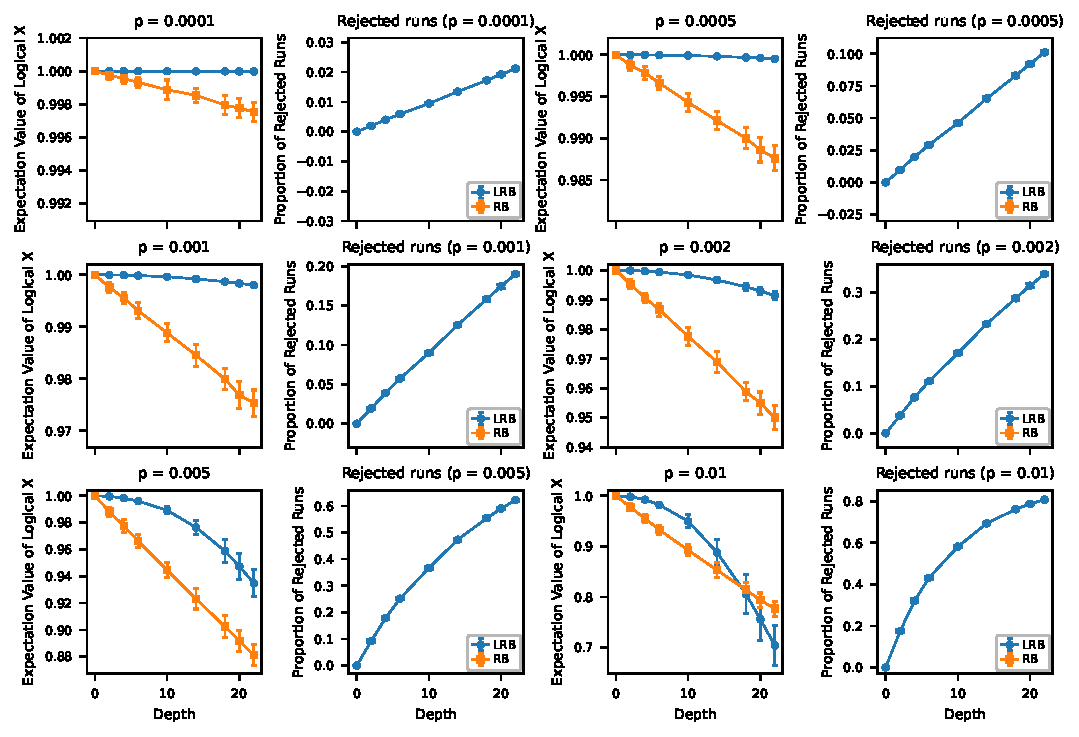
\includegraphics[width=0.95\textwidth]{figures/sdim140/si1000-1anc-const-0-nofit.pdf}
  \caption{Terminal postselection (const-0), one-ancilla layout, SI1000, at six values of $p$ from $10^{-4}$ to $10^{-2}$. In each pair of panels, the left panel shows the accepted $\langle \bar{X} \rangle$ of LRB-D (blue) and $\langle Z \rangle$ of physical RB under SI1000 at the same $p$ (orange) versus depth $m$, and the right panel shows the fraction of rejected LRB-D shots. The axis label ``Expectation Value of Logical X'' refers to LRB-D; for physical RB the plotted quantity is $\langle Z \rangle$. Error bars on $\langle \bar{X} \rangle$ and $\langle Z \rangle$ are standard deviations over the 30 sequences, and error bars on the rejected fraction are standard errors. The legend of each pair sits in its right panel and labels the curves of the left panel. Physical RB rejects no shots, so the right panel shows only LRB-D. No fits are drawn, since the LRB-D traces are not single exponentials.}
  \label{fig:const0_si1000_1anc}
\end{figure}

\begin{figure}[tb]
  \centering
  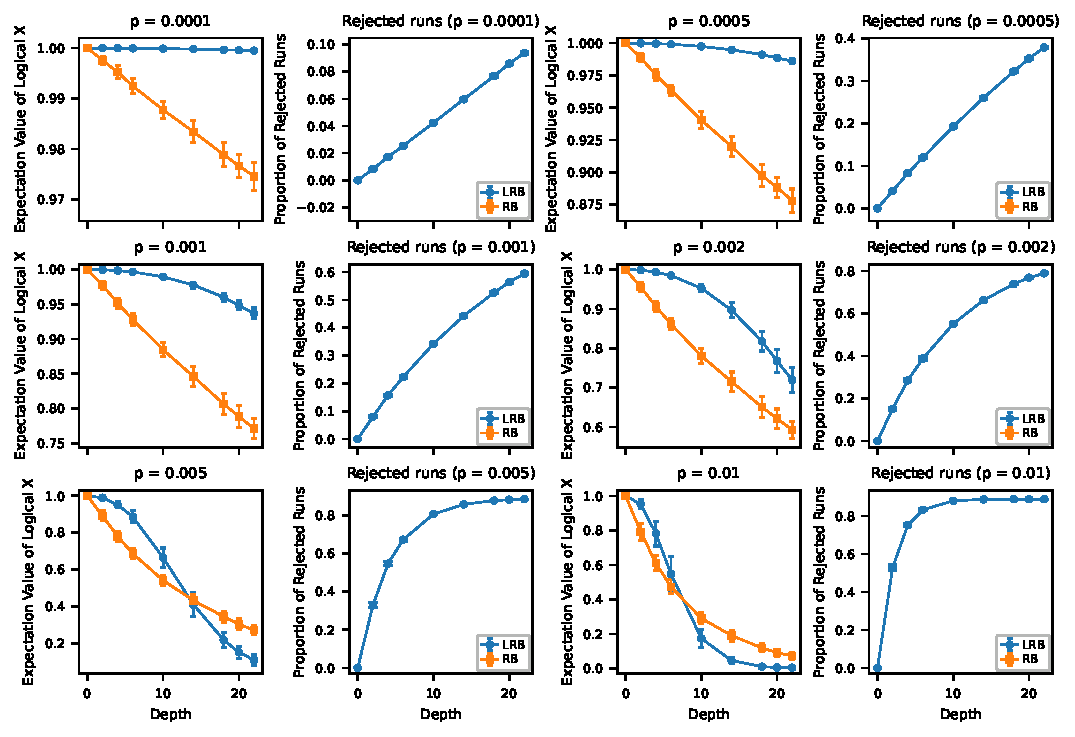
\includegraphics[width=0.95\textwidth]{figures/sdim140/sd6-1anc-const-0-nofit.pdf}
  \caption{Terminal postselection (const-0), one-ancilla layout, SD6, with panels as in \autoref{fig:const0_si1000_1anc}. The RB baseline runs under SD6 at the same $p$. At large $p m$ the rejected fraction approaches $8/9$, the value for uniformly random $X$-type syndromes, and the accepted $\langle \bar{X} \rangle$ approaches zero.}
  \label{fig:const0_sd6_1anc}
\end{figure}

The LRB-D traces stay flat at small depth and then bend down. At small $p$ the deficit $1 - \langle \bar{X} \rangle$ grows quadratically in both $m$ and $p$. Under SI1000 at $p = 10^{-3}$ it is $1.7\times10^{-5}$ at $m = 2$, $3.7\times10^{-4}$ at $m = 10$ and $2.0\times10^{-3}$ at $m = 22$. From $m = 2$ to $m = 10$ it grows by a factor of 22, while the RB deficit grows by a factor of 4.6, from $2.4\times10^{-3}$ to $1.1\times10^{-2}$. At $m = 10$, doubling $p$ from $5\times10^{-4}$ to $10^{-3}$ multiplies the LRB-D deficit by 4.0. SD6 behaves the same way. At $p = 10^{-3}$ the deficit grows by a factor of 28 from $m = 2$ to $m = 10$, from $3.8\times10^{-4}$ to $1.06\times10^{-2}$. Second-order growth in $p$ means that, to leading order, an accepted shot with a wrong readout carries two faults. This is what one expects if every single fault that changes the $X$-basis readout also leaves a nontrivial $X$-type syndrome, so that an accepted failure needs a second fault that restores trivial syndromes while leaving a logical error.

The shape of the traces also bears on the representation-theoretic picture of \autoref{sub:irreps}. Because $\langle \bar{X} \rangle = 1$ at $m = 0$, a single decay mode would give $1 - \langle \bar{X} \rangle \approx m(1-f)$ at small depth, which is linear in $m$. A quadratic onset requires several modes whose first-order contributions cancel. The encoded twirled channel has $m_{triv} + m_{pauli} = 2542$ relevant eigenvalues instead of two, and without intermediate checks one fault can carry the state into a syndrome sector from which a later fault returns it to trivial syndromes with a logical error. The data do not resolve individual modes. They show only that one mode does not describe terminal postselection, and we therefore extract no decay rate from it.

The rejected fraction grows with $m$ and $p$. Under SI1000 at $p = 5\times10^{-3}$ it is 9.2\% at $m = 2$, 37\% at $m = 10$ and 62\% at $m = 22$. Under SD6 it saturates near $8/9 \approx 0.889$, the value expected when the two $X$-type syndromes are uniformly distributed over their nine joint outcomes and only one outcome is accepted. At $p = 10^{-2}$ and $m = 22$ the rejected fraction is 0.8889, and the accepted shots retain almost no logical information, with $\langle \bar{X} \rangle = 0.0048$.

Because the LRB-D deficit grows faster than linearly in $m$ while the RB deficit grows linearly, the accepted $\langle \bar{X} \rangle$ falls below the RB $\langle Z \rangle$ at a depth that shrinks as $p$ grows. Under SI1000 the LRB-D value lies below RB at $m = 22$ for every $p \ge 10^{-2}$, but not at $7.5\times10^{-3}$, and at $m = 10$ for every $p \ge 2\times10^{-2}$, but not at $1.5\times10^{-2}$. Under SD6 it lies below RB at $m = 22$ for every $p \ge 5\times10^{-3}$, but not at $2\times10^{-3}$, and at $m = 10$ for every $p \ge 7.5\times10^{-3}$, but not at $5\times10^{-3}$.

Terminal postselection decays much faster under SD6 than under SI1000. At $p = 10^{-3}$ and $m = 22$ the LRB-D deficit is $6.3\times10^{-2}$ under SD6 and $2.0\times10^{-3}$ under SI1000, a factor of 32. The expected number of faults in a logical Clifford grows by a factor of five from SI1000 to SD6 ($5.7p$ to $29p$), and with second-order failures this alone predicts a factor of about 25. The RB baseline degrades as well, from a deficit of $0.025$ to $0.229$ at the same point.

\subsection{Uniform-Interval Postselection}
\label{sub:interval_results}

Under uniform-interval postselection with interval $k$, a shot is kept only if the check rounds after forward Cliffords $k, 2k, \dots$ and the final round all return trivial syndromes. The check round after every forward Clifford is present for every $k$, so all schedules share the same circuits and the same noise and differ only in the filter. For every $k$ the $m$ inverse Cliffords run without intermediate checks and are filtered only by the final round.

\paragraph{Interval $k = 1$.}
\autoref{fig:unif1_si1000_1anc} and \autoref{fig:unif1_sd6_1anc} show $k = 1$ in the one-ancilla layout. The accepted $\langle \bar{X} \rangle$ decays slowly. Under SI1000 the zero-offset fits follow the data closely, with $\chi^2 = 0.29$ and $0.43$ over nine depths at $p = 10^{-3}$ and $5\times10^{-3}$. Here $\chi^2$ is the weighted sum of squared residuals, with weights set by the variance over sequences rather than the variance of the mean, and it is not divided by the number of degrees of freedom. We use it only to compare schedules at the same $p$. Under SD6 the fits are worse at small $p$, with $\chi^2 = 6.6$ at $p = 10^{-3}$ and $15$ at $2\times10^{-3}$ over nine depths. The decay steepens with depth. At $p = 10^{-3}$, $\langle \bar{X} \rangle$ drops by $6.6\times10^{-5}$ per unit depth between $m = 0$ and $6$ and by $3.0\times10^{-4}$ per unit depth between $m = 18$ and $22$. This is consistent with the unfiltered inverse half, in which pairs of faults accumulate quadratically in $m$ as under terminal postselection, and with the five times larger fault budget of an SD6 logical Clifford. Frequent filtering thus removes most of the syndrome memory behind the multi-mode behavior of \autoref{sub:terminal_results}, but not all of it.

\begin{figure}[tb]
  \centering
  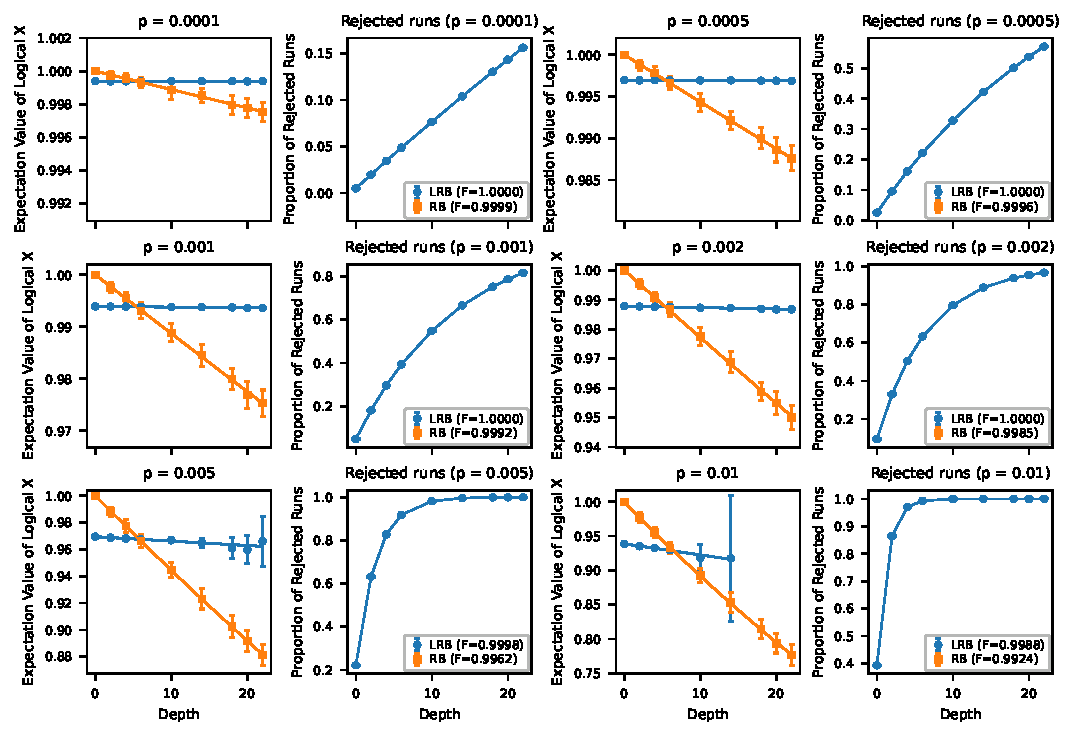
\includegraphics[width=0.95\textwidth]{figures/sdim140/si1000-1anc-unif-1-fit.pdf}
  \caption{Uniform-interval postselection with interval $k = 1$, one-ancilla layout, SI1000. Panels and error bars as in \autoref{fig:const0_si1000_1anc}. The lines are zero-offset fits $F(m) = A f^m$ to LRB-D (blue) and RB (orange), and the legends in the right panels give $\bar{F}$ per unit of depth. Missing LRB-D points at large $m$ and $p$ are depths at which some sequence keeps no shot.}
  \label{fig:unif1_si1000_1anc}
\end{figure}

\begin{figure}[tb]
  \centering
  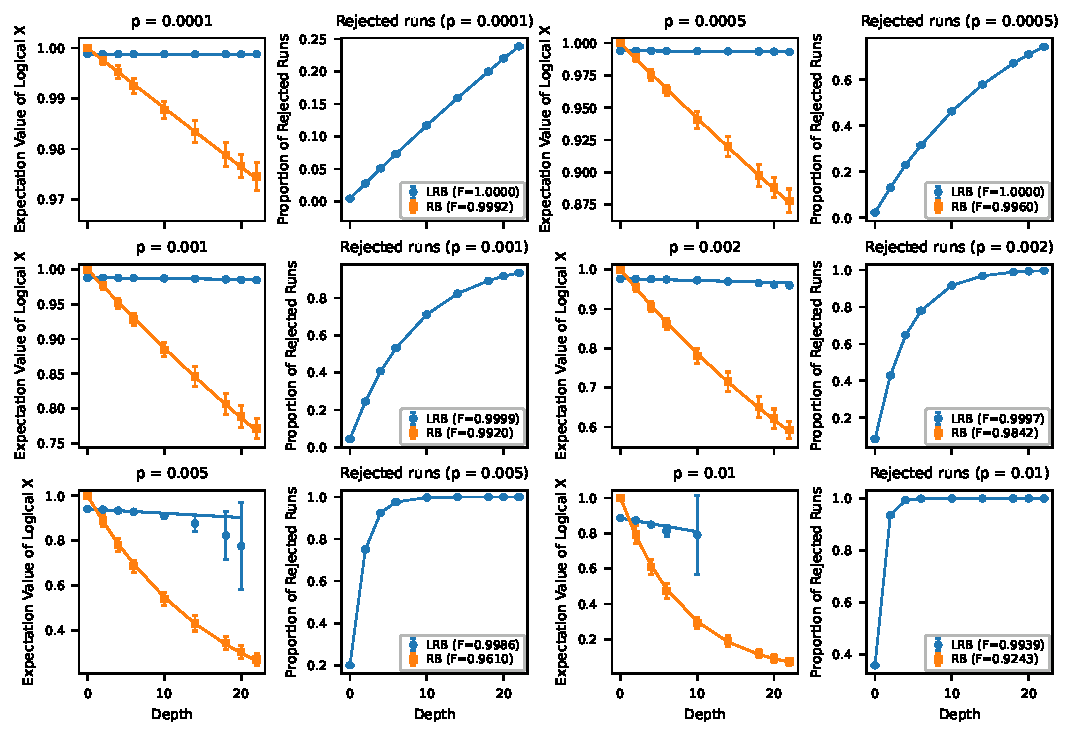
\includegraphics[width=0.95\textwidth]{figures/sdim140/sd6-1anc-unif-1-fit.pdf}
  \caption{Uniform-interval postselection with interval $k = 1$, one-ancilla layout, SD6, with panels, fits and legends as in \autoref{fig:unif1_si1000_1anc}. The RB baseline runs under SD6 at the same $p$, so its gates fail with probability $p$ and it decays ten times faster than under SI1000.}
  \label{fig:unif1_sd6_1anc}
\end{figure}

\autoref{tab:k1_error_rates} compares the fitted error rates with RB at four values of $p$. At $p = 5\times10^{-3}$ the average logical fidelity per unit depth is $\bar{F} = 0.99977$ against $0.9962$ for RB under SI1000, and $0.9986$ against $0.961$ under SD6. Between $p = 5\times10^{-4}$ and $2\times10^{-3}$ the LRB-D error grows as $p^{2.0}$ under SI1000 and $p^{1.9}$ under SD6, while the RB error grows as $p^{1.0}$ under both. Quadratic scaling is what one expects from a distance-2 code with postselection, since an accepted logical error needs two faults. The ratio $r_{\mathrm{RB}}/r_{\mathrm{LRB}}$ falls from 92 (SI1000) and 96 (SD6) at $p = 10^{-3}$ to 2.1 and 4.3 at $p = 2\times10^{-2}$. Under SD6 this is close to $1/p$. Under SI1000 the ratio falls faster, roughly as $p^{-1.3}$, because there the LRB-D error grows faster than $p^2$ above $p = 5\times10^{-3}$, as $p^{2.4}$ to $10^{-2}$ and $p^{2.6}$ from there to $2\times10^{-2}$.

\begin{table}[H]
  \centering
  \small
  \begin{tabular}{c|ccc|ccc}
    \hline
    & \multicolumn{3}{c|}{SI1000} & \multicolumn{3}{c}{SD6} \\
    $p$ & $r_{\mathrm{LRB}}$ & $r_{\mathrm{RB}}$ & depths & $r_{\mathrm{LRB}}$ & $r_{\mathrm{RB}}$ & depths \\
    \hline
    $10^{-3}$ & $(8.3 \pm 0.8)\times10^{-6}$ & $7.6\times10^{-4}$ & 9 & $(8.26 \pm 0.18)\times10^{-5}$ & $8.0\times10^{-3}$ & 9 \\
    $5\times10^{-3}$ & $(2.27 \pm 0.12)\times10^{-4}$ & $3.8\times10^{-3}$ & 9 & $(1.38 \pm 0.04)\times10^{-3}$ & $3.9\times10^{-2}$ & 8 \\
    $10^{-2}$ & $(1.16 \pm 0.04)\times10^{-3}$ & $7.6\times10^{-3}$ & 6 & $(6.05 \pm 0.20)\times10^{-3}$ & $7.6\times10^{-2}$ & 5 \\
    $2\times10^{-2}$ & $(7.15 \pm 0.24)\times10^{-3}$ & $1.5\times10^{-2}$ & 4 & $(3.29 \pm 0.21)\times10^{-2}$ & $1.4\times10^{-1}$ & 3 \\
    \hline
  \end{tabular}
  \caption{Fitted error rates per unit of depth for LRB-D with $k = 1$ in the one-ancilla layout ($r_{\mathrm{LRB}}$, with bootstrap standard deviation) and for physical RB under the same model at the same $p$ ($r_{\mathrm{RB}}$). The columns ``depths'' give the number of depths in the LRB-D fit. All values come from the production runs, and all RB fits use nine depths.}
  \label{tab:k1_error_rates}
\end{table}

The LRB-D traces start below one. At $m = 0$ the circuit consists of the ideal preparation, one noisy check round and the ideal readout. The accepted $\langle \bar{X} \rangle$ at $m = 0$ is $0.9939$, $0.9695$ and $0.9387$ at $p = 10^{-3}$, $5\times10^{-3}$ and $10^{-2}$ under SI1000, and $0.9881$, $0.9415$ and $0.8856$ under SD6. The deficit is first order in $p$, about $6p$ under SI1000 and $12p$ under SD6. It comes from faults on the data qutrits after their last two-qutrit gate of the round, including the idle noise during the final readout moment. A fault there that changes the logical readout leaves every syndrome of the round trivial, and no later round follows. Every depth ends with the same final round, so this loss enters as a common factor that the fitted amplitude absorbs ($A = 0.9695$ under SI1000 at $p = 5\times10^{-3}$), and to leading order it does not bias $f$. Because the RB trace starts at one, the raw curves cross at small depth, between $m = 4$ and $6$ under SI1000 at $p = 5\times10^{-3}$, although the LRB-D decay there is 17 times slower. We therefore compare decay rates rather than raw values.

The price of $k = 1$ is a fast-growing rejection. Under SI1000 at $p = 5\times10^{-3}$, 22\% of the shots are rejected at $m = 0$, 63\% at $m = 2$, 98.1\% at $m = 10$ and 99.98\% at $m = 22$, which leaves about 200 of $10^6$ shots per sequence. At $p = 10^{-3}$ the rejected fractions at the same depths are 4.9\%, 18\%, 55\% and 82\%. Under SD6 at $p = 5\times10^{-3}$ they are 20\% at $m = 0$, 75\% at $m = 2$ and 99.8\% at $m = 10$, and at $m = 22$ some sequence keeps no shot.

\paragraph{Intervals $k = 2$ to $4$ and beyond.}
\autoref{fig:unif2_si1000_1anc} to \autoref{fig:unif4_sd6_1anc} in \autoref{sec:additional-results} show $k = 2$, $3$ and $4$ in the one-ancilla layout. Fewer filters raise both the acceptance and the error per unit depth. Under SI1000 at $p = 5\times10^{-3}$, the rejected fraction at $m = 10$ falls from 98.1\% at $k = 1$ to 96.0\%, 94.6\% and 93.7\% at $k = 2$, $3$ and $4$, while the fitted LRB-D error rises from $2.3\times10^{-4}$ to $3.9\times10^{-4}$, $6.6\times10^{-4}$ and $9.3\times10^{-4}$. Under SD6 at the same $p$ the error rises from $1.4\times10^{-3}$ to $2.0\times10^{-3}$, $3.8\times10^{-3}$ and $5.3\times10^{-3}$.

Under SI1000 the fit quality changes in a step between $k = 2$ and $k = 3$. At $p = 5\times10^{-3}$, $\chi^2$ is $0.43$, $0.39$, $12.6$ and $9.1$ for $k = 1$ to $4$, all over nine depths. Under SD6, $\chi^2$ already exceeds 4 at $k = 1$ and grows more gradually with $k$, as $4.8$ (eight depths), $7.5$, $14.8$ and $24.8$ at the same $p$. The SI1000 step has a structural origin. For $k = 1$ and $2$ every depth of the production grid is a multiple of $k$, so the last forward Clifford is always followed by a filtered round. For $k \ge 3$ the number $m \bmod k$ of forward Cliffords after the last filtered intermediate round varies irregularly along the grid, as $0, 2, 1, 0, 1, 2, 0, 2, 1$ for $k = 3$, and the accepted $\langle \bar{X} \rangle$ develops small steps, so that a single exponential describes it only approximately. Under SD6 at $p = 10^{-3}$ and $k = 3$, for example, $\langle \bar{X} \rangle$ drops by $1.8\times10^{-4}$ from $m = 14$ to $18$, where this count falls from 2 to 0, and by $2.2\times10^{-3}$ from $m = 18$ to $20$, where it rises to 2. The second drop spans half the depth of the first and is twelve times larger, while the standard errors of these points are about $10^{-4}$. The extension runs also contain the odd depths $1$ and $3$, at which the $k = 2$ traces show the same steps, and their $k \ge 2$ fits therefore use only the even depths (\autoref{sub:pseudo_thresholds}).

Beyond $k = 4$, $\chi^2$ keeps growing. At $p = 5\times10^{-3}$ it reaches $116$ at $k = 10$ and $1213$ at $k = 22$ under SI1000, and $217$ and $3522$ under SD6, all over nine depths. Large intervals approach the case of a single filtered round at the end of the sequence, and the traces inherit the multi-mode behavior of terminal postselection. A fit to Eq.~\eqref{eq:fseq} then summarizes the trend but no longer estimates a logical error rate, so we restrict the quantitative analysis to $k \le 4$.

\paragraph{Fits at large $p$.}
In the production runs, the LRB-D fits rest on few depths from $p = 0.02$ on, because at larger depths some sequence keeps no shot. There the $k = 1$ fits use four depths at $p = 0.02$, three at $0.03$ and two at $0.04$ under SI1000, and three at $0.02$ and two at $0.03$ under SD6. The extension runs, at $p \ge 0.015$ under SI1000 and $p \ge 0.025$ under SD6, have more shots per depth but stop at $m = 6$, and their $k = 1$ fits use four to six depths under SI1000 and three to five under SD6. Unless $f$ reaches its bound of one, a two-point fit passes through both points exactly ($\chi^2 < 10^{-9}$). It says nothing about whether the decay is exponential, and its bootstrap interval reflects only the statistical errors of the two points. In addition, the per-sequence modulus $\lvert P_0 + \omega P_1 + \omega^2 P_2 \rvert$ is biased upward when only a few shots survive, since it is positive even for uniformly random outcomes. Under SD6 with $k = 4$ at $p = 0.02$, for example, the point at $m = 10$ rests on an average of 3.6 accepted shots per sequence and gives $\langle \bar{X} \rangle = 0.55$, above the value $0.39$ at $m = 2$. Error rates of the production runs at $p \ge 0.02$, and the SD6 pseudo-thresholds whose bracketing fits rest on few depths (\autoref{sub:pseudo_thresholds}), carry this systematic caveat in addition to their bootstrap errors.

\subsection{Pseudo-Thresholds}
\label{sub:pseudo_thresholds}

For each interval $k$ we define the pseudo-threshold $p^\star(k)$ as the value of $p$ at which the fitted LRB-D error rate equals the fitted error rate of physical RB under the same noise model. Below $p^\star(k)$ the postselected logical qutrit has the lower error per unit depth. In practice we locate $p^\star(k)$ as the onset of the regime in which the LRB-D error stays at or above the RB error, within a tolerance of $5\times10^{-4}$, at every larger $p$ on the grid, and we interpolate the difference linearly between the two bracketing grid points. The search skips the lowest grid points, where both error rates are below $2\times10^{-3}$. Before the search we cut the high-$p$ tail at the first point where the fitted LRB-D error drops below its running maximum by more than $0.01$ or 25\%, whichever is larger, since such drops come from fits starved of accepted shots. For both models the search runs on the merged grids of \autoref{sub:results_setup}, with the production fits at $p < p_{\mathrm{split}}$ and the extension fits from $p_{\mathrm{split}}$ to $0.05$ (SI1000, $p_{\mathrm{split}} = 0.015$) or $0.06$ (SD6, $p_{\mathrm{split}} = 0.025$). For $k \ge 2$ the extension fits use only the even depths $m = 0$, $2$, $4$ and $6$, for the reason given below. The uncertainty of $p^\star(k)$ is one standard error from the bootstrap over the random Clifford sequences of \autoref{sub:fit_model}, with 1000 replicates. Each replicate resamples the sequences of the production and extension runs, LRB-D and RB alike, refits every curve, and repeats the search described here, tail cut included.

% Bracketing fits, depth counts and accepted shots: paper-rework/scratch/writer-conv/analysis.py (sections A, A2); its lib.py applies the even-depth rule and reproduces all 16 canonical values (section V) of LRB-experiment-data-slurm/comparisons/pseudo-thresholds-current.csv (one-ancilla rows) and pseudo-thresholds-conv-sites-current.csv (two-ancilla rows)
\autoref{tab:pseudo_thresholds} lists $p^\star(k)$ for the four configurations. All sixteen entries are genuine crossings, bracketed by grid points at which the LRB-D error is below and above the RB error, and we quote them with one standard error from the sequence bootstrap. Every LRB-D fit that brackets an SI1000 crossing uses four to eight depths, and under SD6 those that bracket $p^\star(1)$ and $p^\star(2)$ use three to five. Near $p^\star(1)$ and $p^\star(2)$ the bracketing fits cover only $m \le 6$. All of them come from the extension, except the lower one for $p^\star(2)$ of the two-ancilla layout under SD6, the production fit at $p = 0.02$ over the depths $0$, $2$ and $4$. The largest depths of some bracketing fits keep few accepted shots (\autoref{sub:postselection_cost}). Under SD6, where these fits rest on as few as three depths, the systematic caveats of \autoref{sub:interval_results} therefore apply. Under SI1000 the few-shot points carry almost no weight in the fit.

Under SI1000 the one-ancilla crossings at $k = 1$, $2$ and $3$ lie between extension points, at $0.0275$ and $0.03$ for $k = 1$, $0.0225$ and $0.025$ for $k = 2$, and $0.015$ and $0.0175$ for $k = 3$, and the crossing at $k = 4$ lies between the production point $0.0125$ and the extension point $0.015$. The two-ancilla crossings lie between the extension points $0.025$ and $0.0275$ for $k = 1$ and $0.02$ and $0.0225$ for $k = 2$, between the production point $0.0125$ and the extension point $0.015$ for $k = 3$, and between the production points $0.01$ and $0.0125$ for $k = 4$. Under SD6 the one-ancilla $p^\star(1)$ lies between the extension points $0.035$ and $0.04$ and $p^\star(2)$ between the extension points $0.025$ and $0.03$. The two-ancilla $p^\star(1)$ lies between the extension points $0.025$ and $0.03$ and $p^\star(2)$ between the production point $0.02$ and the extension point $0.025$. The SD6 values at $k = 3$ and $4$ lie between production grid points, and the extension only confirms that the LRB-D error stays above RB beyond them.

\begin{table}[htb]
  \centering
  \begin{tabular}{c|cc|cc}
    \hline
    & \multicolumn{2}{c|}{one-ancilla layout} & \multicolumn{2}{c}{two-ancilla layout} \\
    $k$ & SI1000 & SD6 & SI1000 & SD6 \\
    \hline
    1 & $0.0292 \pm 0.0006$ & $0.0399 \pm 0.0015$ & $0.0266 \pm 0.0004$ & $0.0283 \pm 0.0007$ \\
    2 & $0.0239 \pm 0.0005$ & $0.0269 \pm 0.0007$ & $0.0209 \pm 0.0003$ & $0.0212 \pm 0.0003$ \\
    3 & $0.0166 \pm 0.0004$ & $0.0181 \pm 0.0006$ & $0.0136 \pm 0.0003$ & $0.0122 \pm 0.0003$ \\
    4 & $0.0132 \pm 0.0002$ & $0.0155 \pm 0.0004$ & $0.0108 \pm 0.0001$ & $0.0103 \pm 0.0001$ \\
    \hline
  \end{tabular}
  \caption{Pseudo-thresholds $p^\star(k)$ against physical RB under the same noise model at the same $p$. Uncertainties are one standard error (68\% confidence), from a bootstrap over the random Clifford sequences (\autoref{sub:fit_model}). All entries are genuine crossings. All entries use the production fits at $p < p_{\mathrm{split}}$ and the high-$p$ extension (depths $0, 1, 2, 3, 4, 6$; $2\times10^7$ shots per sequence and depth; 30 new sequences) at $p \ge p_{\mathrm{split}}$, with $p_{\mathrm{split}} = 0.015$ under SI1000 and $0.025$ under SD6. For $k \ge 2$ the extension fits use only the even depths $0, 2, 4, 6$, as in the production grid, which removes the odd depths at which the $k = 2$ traces show steps. Where production and extension overlap, their fitted RB errors differ by 3.1 to 4.6\% under SI1000 and by 3.8 to 9.4\% under SD6 (\autoref{sub:results_setup}).}
  \label{tab:pseudo_thresholds}
\end{table}

% Even-depth rule: applied by scripts/merge_highp_threshold_extension.py (class EvenDepthsForSparseChecks)
The extension fits for $k \ge 2$ use only even depths because of the steps described in \autoref{sub:interval_results}. At a depth that is not a multiple of $k$, the last $m \bmod k$ forward Cliffords run without a filtered round before the final round (one Clifford at the odd depths for $k = 2$), so the accepted $\langle \bar{X} \rangle$ at such depths lies on a different curve. For $k = 2$ these are the odd depths $1$ and $3$ of the extension grid. All production depths are even, so the rule gives both data sets the same depth structure. For $k = 3$ and $4$ the even depths still include depths that are not multiples of $k$, $m = 2$ and $4$ for $k = 3$ and $m = 2$ and $6$ for $k = 4$, as the production grid does.

% Fit quality near the SI1000 crossings: lrb_chi2 / (lrb_n_points - 2) of the merged tables, LRB-experiment-data-slurm/comparisons/sdim140-si1000-highp-merged/one-ancilla-si1000/ and sdim140-conv-sites-si1000-highp-merged/conv-two-ancilla-si1000/unif_lrb_vs_rb_table_merged.csv, p = 0.015 to 0.035: paper-rework/scratch/writer-conv/analysis.py (section X)
Near the SI1000 crossings the single-exponential fits still describe the accepted decays well at $k = 1$ and $2$. Between $p = 0.015$ and $0.035$ their $\chi^2$ per degree of freedom, defined as in \autoref{sub:interval_results}, is $0.1$ to $1.1$ in both layouts. At $k = 3$ and $4$ it is $1.3$ to $9.6$, because of the steps at depths that are not multiples of $k$.

\autoref{fig:threshold_grid_si1000_1anc} and \autoref{fig:threshold_grid_sd6_1anc} show the construction for the one-ancilla layout, and \autoref{fig:pstar_vs_k} collects $p^\star(k)$ for all four configurations. The corresponding two-ancilla figures are \autoref{fig:threshold_grid_si1000_2anc} and \autoref{fig:threshold_grid_sd6_2anc}.

\begin{figure}[htb]
  \centering
  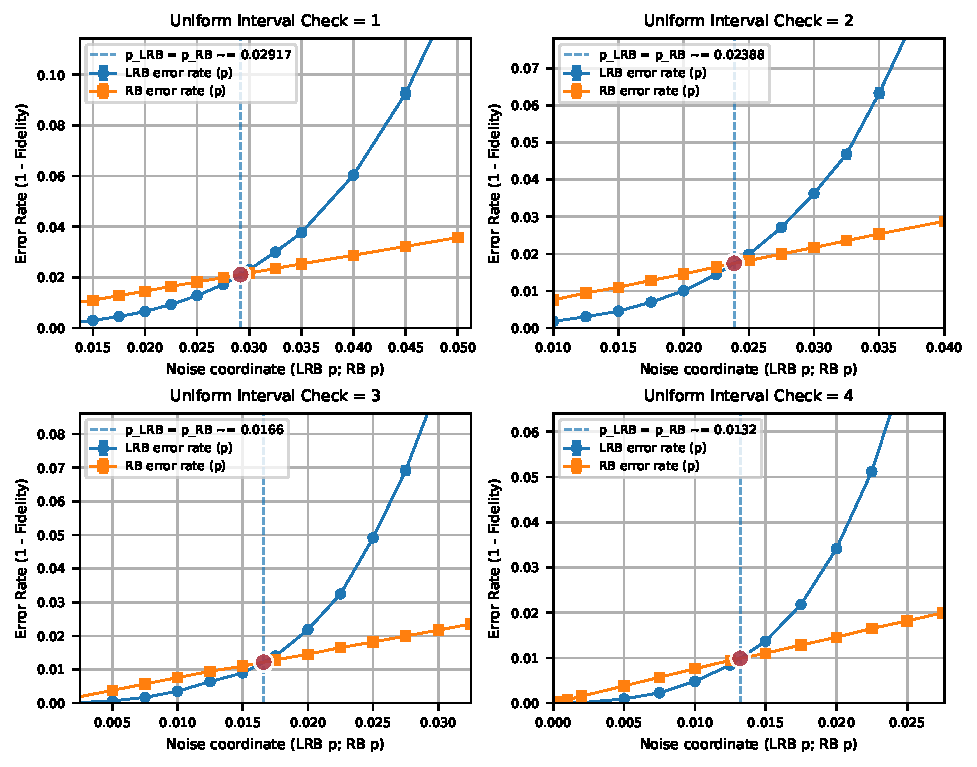
\includegraphics[width=0.75\textwidth]{figures/sdim140/si1000-1anc-threshold-grid.pdf}
  \caption{Pseudo-threshold construction, one-ancilla layout, SI1000. Fitted error rate per unit of depth of LRB-D (blue) and of physical RB under SI1000 at the same $p$ (orange) versus $p$, for $k = 1$, $2$, $3$ and $4$, with 68\% bootstrap intervals. Points at $p < 0.015$ come from the production run, and points at $p \ge 0.015$ from the high-$p$ extension. There the $k = 1$ fits use those of the depths $0, 1, 2, 3, 4$ and $6$ at which every sequence keeps at least one shot, four to six depths, and the $k \ge 2$ fits use the even depths $0, 2, 4$ and $6$, three or four depths (\autoref{sub:results_setup}). The $k = 1$ panel shows only extension points. The vertical line and the marker give $p^\star(k) = 0.0292$, $0.0239$, $0.0166$ and $0.0132$, all genuine crossings. The RB error rises about linearly in $p$, and the LRB-D error rises faster and crosses it. The $k = 1$, $2$ and $3$ crossings lie between extension points, and the $k = 4$ crossing lies between the production point $0.0125$ and the extension point $0.015$. The fits that bracket $p^\star(1)$ use six depths, and those that bracket $p^\star(2)$ and $p^\star(3)$ use four. For $k = 4$ the production fit at $p = 0.0125$ uses seven depths and the extension fit at $0.015$ uses four.}
  \label{fig:threshold_grid_si1000_1anc}
\end{figure}

\begin{figure}[htb]
  \centering
  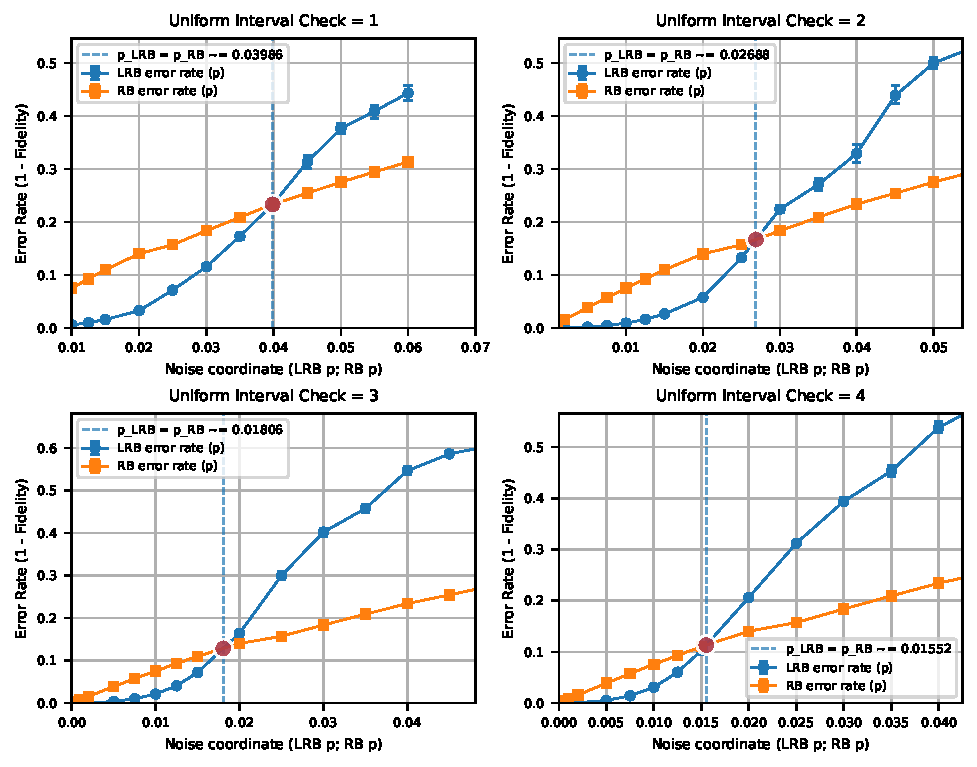
\includegraphics[width=0.75\textwidth]{figures/sdim140/sd6-1anc-threshold-grid.pdf}
  \caption{Pseudo-threshold construction, one-ancilla layout, SD6, with curves as in \autoref{fig:threshold_grid_si1000_1anc} and RB under SD6. Points at $p < 0.025$ come from the production run, and points at $p \ge 0.025$ from the high-$p$ extension. There the $k = 1$ fits use those extension depths at which every sequence keeps at least one shot, three to five depths with $m \le 4$, and the $k \ge 2$ fits use three or four of the even depths $0, 2, 4$ and $6$ (\autoref{sub:results_setup}). The markers are genuine crossings at $p^\star(k) = 0.0399$, $0.0269$, $0.0181$ and $0.0155$. The $k = 1$ and $2$ crossings lie between extension points, and the $k = 3$ and $4$ crossings between production points.}
  \label{fig:threshold_grid_sd6_1anc}
\end{figure}

\begin{figure}[htb]
  \centering
  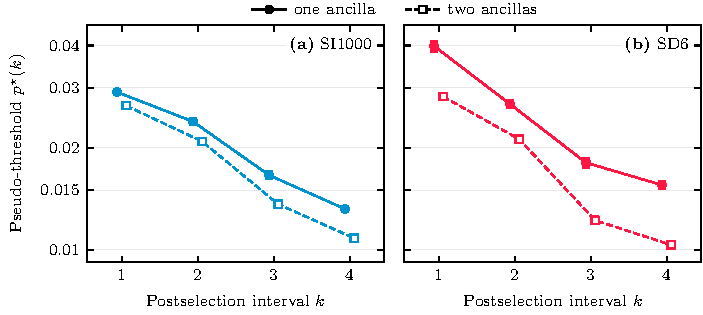
\includegraphics{figures/sdim140/pstar-vs-k.pdf}
  \caption{Pseudo-threshold $p^\star(k)$ versus postselection interval $k$ under (a)~SI1000 and (b)~SD6, for the one-ancilla layout (filled circles, solid lines) and the two-ancilla layout (open squares, dashed lines). All points are genuine crossings of the LRB-D and RB error rates. Error bars are one standard error (68\% confidence) from the bootstrap over the random Clifford sequences (\autoref{sub:fit_model}); bars that are not visible are smaller than the markers. All values use the production fits at $p < p_{\mathrm{split}}$ and the high-$p$ extension at $p \ge p_{\mathrm{split}}$, with $p_{\mathrm{split}} = 0.015$ under SI1000 and $0.025$ under SD6, and for $k \ge 2$ only the even extension depths (\autoref{sub:results_setup}). For legibility the two layouts are drawn $0.06$ to the left and right of each $k$, and the lines guide the eye.}
  \label{fig:pstar_vs_k}
\end{figure}

% Factors from LRB-experiment-data-slurm/comparisons/pseudo-thresholds-current.csv; paired adjacent-interval gaps: LRB-experiment-data-slurm/comparisons/sequence-bootstrap/interval_gap_significance.csv (one-ancilla rows, checked from the replicate files by paper-rework/scratch/writer-seq-se/paired.py, paired.out) and interval_gap_significance-conv-sites.csv (conv-two-ancilla rows); SD6-versus-SI1000 ratios with relative standard errors in quadrature: paper-rework/scratch/writer-conv/analysis.py (sections S3, S4), from pseudo-thresholds-current.csv (one-ancilla rows) and pseudo-thresholds-conv-sites-current.csv
In every configuration $p^\star(k)$ falls with $k$. The decrease of $p^\star$ with the check interval is significant at 6 standard errors or more for every adjacent pair of intervals, with the bootstrap replicates paired over the shared sequences, whose common fluctuations largely cancel in the differences. The smallest steps, from $k = 3$ to $4$ under SD6, amount to 6.1 standard errors with one ancilla and 6.6 with two, and the ordering $p^\star(1) > p^\star(2) > p^\star(3) > p^\star(4)$ holds in all 1000 replicates of every configuration. In the one-ancilla layout it drops by a factor of 2.2 from $k = 1$ to $4$ under SI1000 ($0.0292$ to $0.0132$) and by a factor of 2.6 under SD6 ($0.0399$ to $0.0155$).
The circuits are identical for all $k$, so the drop reflects only which shots are kept. A fault that a skipped round would have flagged survives until the next filtered round. If a second fault arrives in between and the two combine into an error with trivial syndromes, for example a logical operator, no later round can detect it. Fewer filters therefore keep more shots that carry logical errors. The fitted LRB-D error at fixed $p$ grows with $k$ (\autoref{sub:interval_results}), while RB does not depend on $k$, and the crossing moves to smaller $p$.
In the one-ancilla layout the factors from $k = 1$ to $2$, $2$ to $3$ and $3$ to $4$ are 1.22, 1.44 and 1.26 under SI1000 and 1.48, 1.49 and 1.16 under SD6.

Here and in \autoref{sub:layout_comparison} we compare two pseudo-thresholds $p^\star_a$ and $p^\star_b$ from independent runs through their ratio. We quote the relative difference $p^\star_a/p^\star_b - 1$ with the standard error of the ratio, which is the ratio times the relative standard errors of $p^\star_a$ and $p^\star_b$ added in quadrature, and its significance is the relative difference divided by this standard error. In the one-ancilla layout, the SD6 pseudo-thresholds lie above the SI1000 values at every $k$. They are $0.0399$ against $0.0292$ at $k = 1$, $0.0269$ against $0.0239$ at $k = 2$, $0.0181$ against $0.0166$ at $k = 3$ and $0.0155$ against $0.0132$ at $k = 4$, higher by $36.7 \pm 5.7\%$, $12.6 \pm 3.7\%$, $8.8 \pm 4.5\%$ and $17.6 \pm 3.8\%$, or 6.5, 3.4, 1.9 and 4.6 standard errors. The ordering is therefore resolved at $k = 1$, $2$ and $4$, and at $k = 3$ only at the level of two standard errors. In the two-ancilla layout the SD6 values are higher by $6.4 \pm 3.1\%$ at $k = 1$ and $1.5 \pm 2.1\%$ at $k = 2$, or 2.0 and 0.7 standard errors, and lower by $10.4 \pm 3.1\%$ at $k = 3$ and $4.6 \pm 1.8\%$ at $k = 4$, or 3.3 and 2.6 standard errors. There the two models give pseudo-thresholds within about 10\% of each other, and only the lower SD6 value at $k = 3$ is resolved at more than three standard errors.

The higher SD6 values of the one-ancilla layout do not mean that the encoded circuits fare better under SD6. At $p = 10^{-2}$ and $k = 1$ the fitted LRB-D error is 5.2 times larger under SD6 than under SI1000 with one ancilla ($6.1\times10^{-3}$ against $1.2\times10^{-3}$) and 8.3 times larger with two ($1.08\times10^{-2}$ against $1.30\times10^{-3}$). The RB baseline is about 10 times worse ($7.6\times10^{-2}$ against $7.6\times10^{-3}$ in the one-ancilla runs and $7.1\times10^{-2}$ against $7.5\times10^{-3}$ in the two-ancilla runs), because its one-qutrit gates fail with probability $p$ instead of $p/10$. A pseudo-threshold thus compares the code with a baseline whose quality depends on the noise model. SI1000 pairs the code with a physical qutrit whose gates are ten times cleaner than the two-qutrit gates that set $p$, and its baseline is the harder one to beat. Whether a layout reaches a higher pseudo-threshold under SD6 then depends on how much more its encoded circuits lose under SD6. With one ancilla the LRB-D error grows by a factor of 5.2, about half the factor of the RB error, and SD6 gives the higher pseudo-thresholds. With two ancillas it grows by a factor of 8.3, close to that of the RB error in the same runs (9.5), and the two models give pseudo-thresholds within about 10\% of each other. This agrees with the noise budget of the longer two-ancilla check round, whose 22 additional idle locations SD6 charges at the full rate $p$ (\autoref{sub:layout_comparison}).

\subsection{One- and Two-Ancilla Layouts}
\label{sub:layout_comparison}

% Gate, moment and idle counts and the noise budget per round: paper-rework/scratch/writer-conv/budget.py (budget.out), from the generator of the conventional-sites worktree; rejected fractions and fitted errors: paper-rework/facts/raw_per_depth.csv and fits_all_k.csv, checked by paper-rework/scratch/writer-conv/analysis.py (sections M, Fk)
The two-ancilla layout measures $G_1$ and $G_4$ with the data relay of \autoref{sub:ancilla_layouts}. Both layouts reset and read out four ancillas per round. The two-ancilla round has 18 two-qutrit gates instead of 12 and 11 gate moments instead of 7, so it occupies 13 moments instead of 9, and in both layouts every two-qutrit gate of the round acts on a data qutrit. The expected number of faults per round rises from $67.9p$ to $76.3p$ under SI1000 and from $73p$ to $103p$ under SD6. Under SI1000, $6p$ of the extra $8.4p$ come from the six additional two-qutrit gates, $2.2p$ from the 22 additional idle locations of the four extra gate moments, which fail with probability $p/10$, and $0.2p$ from the two additional one-qutrit gates. Under SD6 the same idle locations fail with probability $p$ and add $22p$ of the extra $30p$. The reset and readout flips, $28p$ per round under SI1000 and $8p$ under SD6, are the same in both layouts.

The two-ancilla layout rejects more shots. With one check round at $m = 0$ and $p = 5\times10^{-3}$, the rejected fraction grows from 22\% to 25\% under SI1000 and from 20\% to 28\% under SD6. \autoref{fig:four_configs} compares the error per unit depth of the four configurations for $k = 1$. Under SI1000 the fitted LRB-D error is 16\% larger with two ancillas than with one at $p = 5\times10^{-3}$ ($2.6\times10^{-4}$ against $2.3\times10^{-4}$) and 12\% larger at $p = 10^{-2}$ ($1.30\times10^{-3}$ against $1.16\times10^{-3}$). Under SD6 it is 56\% larger at $p = 5\times10^{-3}$ ($2.16\times10^{-3}$ against $1.38\times10^{-3}$) and 78\% larger at $p = 10^{-2}$ ($1.08\times10^{-2}$ against $6.1\times10^{-3}$), from fits over six and four depths with two ancillas and over eight and five with one.

\begin{figure}[htb]
  \centering
  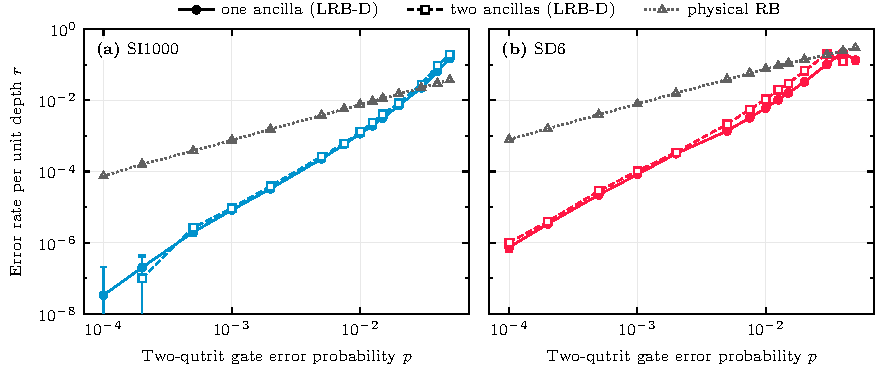
\includegraphics{figures/sdim140/lrb-vs-rb-k1.pdf}
  \caption{Fitted error rate per unit depth $r$ for LRB-D with $k = 1$ (a filtered check round after every forward Clifford) versus $p$ under (a)~SI1000 and (b)~SD6, for the one-ancilla (filled circles, solid lines) and two-ancilla (open squares, dashed lines) layouts, with physical RB under the same noise model (open triangles, dotted lines). One unit of depth is a forward logical Clifford with its mirror inverse (\autoref{sub:fit_model}). The RB points come from the one-ancilla runs. The two-ancilla runs draw their own RB sequences, whose errors differ from these by up to 7.5\% (\autoref{sub:results_setup}). Error bars are central 68\% intervals of the parametric bootstrap (\autoref{sub:fit_model}); bars that are not visible are smaller than the markers, and the intervals that reach zero, under SI1000 at $p \le 2\times10^{-4}$, run to the bottom of the axis. At small $p$ the LRB-D errors scale as $p^2$ and the RB errors as $p$. At $p = 10^{-4}$ the one-ancilla SI1000 value, $3\times10^{-8}$, is one step of the fitted fidelity's numerical resolution, and the two-ancilla SI1000 fit returns zero error and is not drawn. From $p = 0.03$ on, the LRB-D fits rest on two or three depths. The downturns of the SD6 curves, at $p = 0.05$ with one ancilla and at $p = 0.04$ with two, come from such fits, and the two-ancilla SD6 fit at $p = 0.05$ returns zero error and is not drawn. All points are fits to the production runs. The pseudo-thresholds of both models replace the production points at $p \ge 0.015$ (SI1000) and $p \ge 0.025$ (SD6) by fits to the high-$p$ extension, which for $k = 1$ use those extension depths at which every sequence keeps at least one shot (\autoref{fig:threshold_grid_si1000_1anc}, \autoref{fig:threshold_grid_sd6_1anc}, \autoref{fig:threshold_grid_si1000_2anc}, \autoref{fig:threshold_grid_sd6_2anc}). Under SI1000 they place the $k = 1$ crossings at $0.0292$ with one ancilla and $0.0266$ with two, and under SD6 at $0.0399$ and $0.0283$. The production points drawn here meet RB at $p = 0.03$ or cross it between $0.02$ and $0.03$, except those of the one-ancilla SD6 run, which stay below RB.}
  \label{fig:four_configs}
\end{figure}

\autoref{tab:pseudo_thresholds} compares the pseudo-thresholds of the two layouts. Each layout is compared with the RB baseline of its own run. In the production runs at $p \ge 5\times10^{-4}$ the RB errors of the two layouts differ by at most 1.3\% under SI1000, while under SD6 that of the two-ancilla run is 3.7 to 7.5\% smaller, and in the extension runs that of the two-ancilla run is 5.7 to 9.0\% larger (\autoref{sub:results_setup}). The standard errors of $p^\star$ include the spread from the choice of the LRB-D and RB sequences, since the bootstrap resamples both (\autoref{sub:fit_model}). Each gap is $1 - p^\star_{\mathrm{two}}/p^\star_{\mathrm{one}}$, with the standard error of the ratio and the significance defined in \autoref{sub:pseudo_thresholds}, so the relative standard errors of the two runs add in quadrature.
% Layout gaps 1 - p*(two)/p*(one) against each run's own RB, with relative standard errors added in quadrature (independent runs), and the difference of the SD6 and SI1000 gaps: paper-rework/scratch/writer-conv/analysis.py (sections S1, S2), from LRB-experiment-data-slurm/comparisons/pseudo-thresholds-current.csv (one-ancilla rows) and pseudo-thresholds-conv-sites-current.csv
Under SI1000 the two-ancilla values lie below the one-ancilla values by $8.8 \pm 2.3\%$, $12.6 \pm 2.2\%$, $17.9 \pm 2.9\%$ and $17.9 \pm 1.6\%$ at $k = 1$ to $4$, or 3.9, 5.6, 6.2 and 10.9 standard errors.
Under SD6 they lie below by $29.0 \pm 3.1\%$, $21.2 \pm 2.3\%$, $32.4 \pm 2.8\%$ and $33.4 \pm 2.1\%$, with $0.0283$ against $0.0399$, $0.0212$ against $0.0269$, $0.0122$ against $0.0181$ and $0.0103$ against $0.0155$, or 9.2, 9.1, 11.6 and 15.8 standard errors.
Every gap is resolved. The two-ancilla layout costs 9 to 18\% of $p^\star$ under SI1000 and 21 to 33\% under SD6. The SD6 gap exceeds the SI1000 gap by $20.2 \pm 3.9$, $8.6 \pm 3.2$, $14.5 \pm 4.0$ and $15.5 \pm 2.7$ percentage points at $k = 1$ to $4$, with the standard errors of the two gaps added in quadrature, or 5.2, 2.7, 3.6 and 5.8 standard errors. The layouts thus differ more under SD6 at $k = 1$, $3$ and $4$, while at $k = 2$ the difference amounts to 2.7 standard errors. We have not tested whether the gap changes with $k$ within one model. Under SI1000 it grows from 9\% at $k = 1$ to 18\% at $k = 3$ and $4$, but the gaps at different $k$ share the sequences of both runs, so their standard errors do not add in quadrature.

That the gap is larger under SD6 at $k = 1$, $3$ and $4$ agrees with the noise budget of the round. Under SI1000 the four extra gate moments cost little, since qutrits that idle in gate moments fail with probability $p/10$, and most of the added noise comes from the six extra two-qutrit gates, all of which act on data qutrits. Under SD6 every qutrit that a moment leaves untouched fails with probability $p$, and the four extra gate moments add $22p$ per round, against $6p$ from the extra two-qutrit gates. In both models the two-ancilla layout also rejects more shots. The extra gates and gate moments come from the data relay, with which the two-ancilla layout measures $G_1$ and $G_4$ (\autoref{tab:conv_round}). The simulations charge the long-range $q_2$--$q_3$ gate of the one-ancilla layout like any other two-qutrit gate, with one DEP2 at probability $p$ and no SWAP routing, so the gaps measure the cost of the data relay and not that of the long-range coupling.

\subsection{Cost of Postselection and Conditional Interpretation}
\label{sub:postselection_cost}

Postselection is what allows us to benchmark the $[[5,1,2]]_3$ code without a decoder. The code detects every single-qutrit error but cannot correct them (\autoref{sub:lrb_d}), and discarding flagged shots avoids committing to a correction rule. The interval $k$ also provides a control that moves the LRB-D traces toward the multi-mode behavior of terminal postselection, as discussed in \autoref{sub:irreps}. Under SI1000 the decay is close to a single exponential at $k \le 2$ and approximately so at $k = 3$ and $4$ (\autoref{sub:interval_results}). Under SD6 it already steepens with depth at $k = 1$ (\autoref{sub:interval_results}).

The drawback is the sampling cost. In the one-ancilla SI1000 configuration with $k = 1$ at $p = 5\times10^{-3}$, about 200 of $10^6$ shots per sequence survive to $m = 22$ (\autoref{sub:interval_results}). Near the pseudo-threshold the cost is higher. In the production run at $p = 3\times10^{-2}$, 77\% of the shots are rejected at $m = 0$ and 99.74\% at $m = 2$, an average of 28 of $10^6$ shots per sequence survives to $m = 4$, and from $m = 6$ on some sequence keeps no shot. The pseudo-thresholds at $k = 1$ and $2$ therefore rest on the extension runs, which sample $2\times10^7$ shots per sequence and depth up to $m = 6$ (\autoref{sub:results_setup}), except for the lower bracketing fit of the two-ancilla $p^\star(2)$ under SD6 (\autoref{sub:pseudo_thresholds}).
% Depth counts and accepted shots of the bracketing fits: paper-rework/scratch/writer-evendepth/analysis.py (section A) for one ancilla, paper-rework/scratch/writer-conv/analysis.py (section A) for both layouts; spread over sequences of the one-ancilla k = 1 data at p = 0.03: paper-rework/scratch/writer-evendepth/extras.py (m = 0 diagnostics) and paper-rework/scratch/s2-physics-reviewer/c_misc.py (standard errors over the 30 sequences)
Under SI1000 the two fits that bracket $p^\star(1) = 0.0292$, at $p = 0.0275$ and $0.03$, use all six extension depths, but at $m = 6$ an average of only 23 and 6.7 shots per sequence survive. The two that bracket $p^\star(2) = 0.0239$, at $p = 0.0225$ and $0.025$, use the four even depths, and about 2300 and 890 shots per sequence survive to $m = 6$. With two ancillas the fits that bracket $p^\star(1) = 0.0266$, at $p = 0.025$ and $0.0275$, use six and five depths, up to $m = 6$ and $m = 4$, where 20 and 480 shots per sequence survive. Those that bracket $p^\star(2) = 0.0209$, at $p = 0.02$ and $0.0225$, use the four even depths, with about 2300 and 770 shots per sequence at $m = 6$. These numbers measure the sampling cost. The few-shot points carry almost no weight in the fit, which weights each depth by the inverse variance over sequences: at $m = 6$ and $p = 0.03$ the one-ancilla $k = 1$ data scatter over sequences with a standard deviation of $0.23$, against $0.005$ to $0.03$ at $m = 1$ to $4$.
Under SD6 the fits that bracket $p^\star(1)$ come from the extension, at $p = 0.035$ and $0.04$ with one ancilla and at $0.025$ and $0.03$ with two, and rest on five and four of its depths in both layouts. Their largest depths also keep few shots. With one ancilla at $p = 0.035$, the point at $m = 4$ rests on an average of 3.8 of $2\times10^7$ shots per sequence and gives $\langle \bar{X} \rangle = 0.68$, above $0.21$ at $m = 3$, which is the upward bias described in \autoref{sub:interval_results}. Larger $k$ lowers the cost. Under SI1000 at $p = 5\times10^{-3}$, $k = 4$ rejects 50\% of the shots at $m = 2$ and 94\% at $m = 10$, against 63\% and 98\% for $k = 1$, at the price of a larger error per unit depth and a lower pseudo-threshold.

LRB-D also reports a conditional quantity. The fitted error per unit depth describes the logical errors that pass every filtered round, that is, how well the logical state is preserved along the accepted trajectories. It is not the unconditional reliability of a computation of depth $m$, which succeeds only with the acceptance probability. It also leaves out the fixed loss at $m = 0$, which the fitted amplitude absorbs. This loss is about $6p$ (SI1000) or $12p$ (SD6) in the one-ancilla layout and about $7p$ or $17p$ in the two-ancilla layout. A comparison of an encoded qutrit with a physical one should therefore quote the error per unit depth together with the acceptance it requires.

\subsection{Comparison with the Qubit \texorpdfstring{$[[5,1,2]]$}{[[5,1,2]]} Code}
\label{sub:qubit_comparison}

% Qubit p* and seq_boot_se: LRB-experiment-data-slurm/comparisons/pseudo-thresholds-qubit-current.csv (qubit-one-ancilla rows only) and pseudo-thresholds-qubit-conv-sites-current.csv; qutrit p*: tab:pseudo_thresholds. Refits, brackets, ratios with relative standard errors in quadrature, paired gaps, layout gaps, RB and LRB-D error ratios at equal p, word lengths: paper-rework/scratch/writer-qubit/analysis.py (analysis.out, sections T1, R1, G1, L0, B1, L1, X3, X4); ratios cross-checked against comparisons/qubit-vs-qutrit-conv-sites/threshold-comparison.csv. Corrector additions (SD6 bracketing shots, fall factors with bootstrap SE, RB all-order estimate, encoded-error ratio per p, qubit rejected fractions): paper-rework/scratch/corrector-qubit-1/corrector.py (corrector.out, sections A to F, I)
We repeat the simulations of this section for the qubit $[[5,1,2]]$ code of \autoref{sub:qubit_code}. The simulations differ only in the local dimension, $q = 2$ instead of $3$, which changes the code, the logical Clifford group, now with $24$ elements, the Pauli channels of the noise models and the estimator. They share the nine wires, the encoding, the physical circuits of the logical gates, the check rounds of both layouts, the rates of the SI1000 and SD6 models, the production grid of \autoref{sub:results_setup}, the mirror inverse and the fits, $m = 0$ included. The analysis differs in two respects (\autoref{sub:qubit_code}). The threshold search has no tolerance and no error floor. On the qutrit grids this rule returns the published values unchanged, so the ratios below compare values found by the same rule. Near-threshold refinement runs take the place of the high-$p$ extension. The physical baseline is single-qubit RB under the same noise model at the same $p$. The qubit pseudo-thresholds combine production and refinement fits, and all other qubit numbers below come from the production runs.

\autoref{tab:pseudo_thresholds_qubit} lists the qubit $p^\star(k)$ and their ratio to the qutrit values of \autoref{tab:pseudo_thresholds}, and \autoref{fig:pstar_qubit_qutrit} shows both. All sixteen qubit entries are genuine crossings that lie between two refinement points. The fits that bracket them use six to nine depths under SI1000 and three to nine under SD6. Under SD6 the largest fitted depth of each bracketing fit keeps an average of 3.6 to 337 accepted shots per sequence, so the systematic caveat of \autoref{sub:interval_results} applies to the qubit SD6 values as well. Under SI1000 these points keep $\langle \bar X \rangle \ge 0.8$, far above the finite-shot floor. Every qubit pseudo-threshold lies below the qutrit value of the same layout, noise model and interval. The qubit and qutrit runs are independent, so we compare them through the ratio defined in \autoref{sub:pseudo_thresholds}. Under SI1000 the ratio $p^\star_{\mathrm{qubit}}/p^\star_{\mathrm{qutrit}}$ is $0.38$, $0.33$, $0.30$ and $0.30$ at $k = 1$ to $4$ with one ancilla and $0.35$, $0.31$, $0.29$ and $0.29$ with two. Under SD6 it is $0.53$, $0.56$, $0.52$ and $0.47$ with one ancilla and $0.50$, $0.47$, $0.50$ and $0.45$ with two. The qubit values are thus lower by 62 to 71\% under SI1000 and by 44 to 55\% under SD6, and every ratio lies more than 16 standard errors below one.

\begin{table}[htb]
  \centering
  \begin{tabular}{cc|cc|cc}
    \hline
    & & \multicolumn{2}{c|}{SI1000} & \multicolumn{2}{c}{SD6} \\
    layout & $k$ & $p^\star_{\mathrm{qubit}}$ & $p^\star_{\mathrm{qubit}}/p^\star_{\mathrm{qutrit}}$ & $p^\star_{\mathrm{qubit}}$ & $p^\star_{\mathrm{qubit}}/p^\star_{\mathrm{qutrit}}$ \\
    \hline
    one ancilla & 1 & $0.0112 \pm 0.0002$ & $0.38 \pm 0.01$ & $0.0210 \pm 0.0008$ & $0.53 \pm 0.03$ \\
    & 2 & $0.0078 \pm 0.0002$ & $0.33 \pm 0.01$ & $0.0151 \pm 0.0005$ & $0.56 \pm 0.02$ \\
    & 3 & $0.00495 \pm 0.00009$ & $0.30 \pm 0.01$ & $0.0094 \pm 0.0003$ & $0.52 \pm 0.02$ \\
    & 4 & $0.00395 \pm 0.00008$ & $0.30 \pm 0.01$ & $0.0072 \pm 0.0002$ & $0.47 \pm 0.02$ \\
    \hline
    two ancillas & 1 & $0.0093 \pm 0.0001$ & $0.35 \pm 0.01$ & $0.0142 \pm 0.0004$ & $0.50 \pm 0.02$ \\
    & 2 & $0.0064 \pm 0.0001$ & $0.31 \pm 0.01$ & $0.0100 \pm 0.0003$ & $0.47 \pm 0.01$ \\
    & 3 & $0.00395 \pm 0.00008$ & $0.29 \pm 0.01$ & $0.0061 \pm 0.0002$ & $0.50 \pm 0.02$ \\
    & 4 & $0.00313 \pm 0.00005$ & $0.29 \pm 0.01$ & $0.0047 \pm 0.0001$ & $0.45 \pm 0.01$ \\
    \hline
  \end{tabular}
  \caption{Pseudo-thresholds $p^\star(k)$ of the qubit $[[5,1,2]]$ code against single-qubit RB under the same noise model at the same $p$, and their ratio to the qutrit values of \autoref{tab:pseudo_thresholds} for the same layout, noise model and interval. Uncertainties are one standard error (68\% confidence), from a bootstrap over the random Clifford sequences (\autoref{sub:fit_model}). The uncertainty of a ratio is the ratio times the relative standard errors of the qubit and qutrit values added in quadrature (\autoref{sub:pseudo_thresholds}). All entries are genuine crossings. They use the production fits outside and the near-threshold refinement fits inside the refinement window of \autoref{sub:qubit_code}, $0.002 \le p \le 0.013$ under SI1000 and $0.006 \le p \le 0.026$ (one ancilla) or $0.003 \le p \le 0.026$ (two ancillas) under SD6. Where production and refinement overlap, their fitted RB errors differ by up to 5.6\% under SI1000 and 4.9\% under SD6 (\autoref{sub:qubit_code}).}
  \label{tab:pseudo_thresholds_qubit}
\end{table}

\begin{figure}[htb]
  \centering
  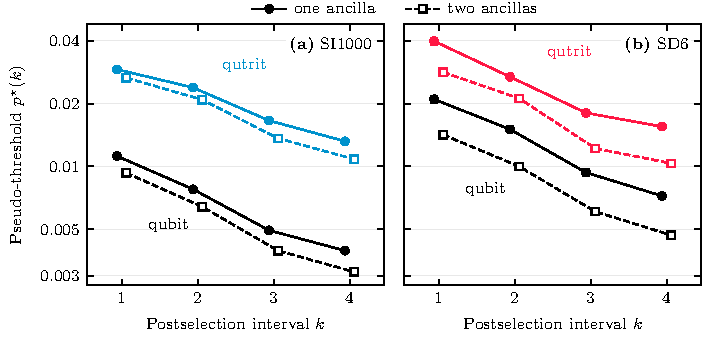
\includegraphics{figures/sdim140/pstar-qubit-vs-qutrit.pdf}
  \caption{Pseudo-threshold $p^\star(k)$ versus postselection interval $k$ for the qutrit (colored) and qubit (black) $[[5,1,2]]$ codes under (a)~SI1000 and (b)~SD6, for the one-ancilla layout (filled circles, solid lines) and the two-ancilla layout (open squares, dashed lines). Each $p^\star$ is the crossing of the LRB-D error rate with the physical RB error rate of the same local dimension under the same noise model. The qutrit points are those of \autoref{fig:pstar_vs_k}. The qubit points combine the qubit production runs with refinement runs near the crossings, on a finer grid of $p$ and at the production depths (\autoref{sub:qubit_code}). All points are genuine crossings. Error bars are one standard error (68\% confidence) from the bootstrap over the random Clifford sequences (\autoref{sub:fit_model}); bars that are not visible are smaller than the markers. For legibility the two layouts are drawn $0.06$ to the left and right of each $k$, and the lines guide the eye.}
  \label{fig:pstar_qubit_qutrit}
\end{figure}

As for the qutrit, $p^\star(k)$ falls with $k$ in every qubit configuration. With the bootstrap replicates paired over the shared sequences, as in \autoref{sub:pseudo_thresholds}, every step between adjacent intervals is significant at 12.1 standard errors or more, and the ordering $p^\star(1) > p^\star(2) > p^\star(3) > p^\star(4)$ holds in all 1000 replicates of every configuration. From $k = 1$ to $4$ the qubit values fall by factors of $2.84 \pm 0.05$ with one ancilla and $2.98 \pm 0.04$ with two under SI1000, and by $2.91 \pm 0.08$ and $3.03 \pm 0.06$ under SD6, against $2.21 \pm 0.04$, $2.45 \pm 0.05$, $2.57 \pm 0.12$ and $2.74 \pm 0.08$ for the qutrit. Each standard error comes from the bootstrap replicates of one configuration, paired over its shared sequences. Compared through their ratio as in \autoref{sub:pseudo_thresholds}, the qubit factors are larger by 8.6 and 7.0 standard errors under SI1000 but only by 2.2 and 2.9 under SD6. The two-ancilla layout also gives the lower qubit values, by 17 to 21\% under SI1000 and 32 to 35\% under SD6, or 7.9 to 12.6 standard errors.

Part of the difference lies in the physical baseline. At the same $p$ the qubit RB error is the smaller one (\autoref{fig:k1_qubit_qutrit}). In the production runs from $p = 5\times10^{-4}$ to $0.05$, it is 0.45 to 0.47 times the qutrit RB error of the same layout under SI1000 and 0.42 to 0.49 times under SD6. The gate counts of the two Clifford groups and the error of a single noisy gate account for this ratio. The RB circuits apply every primitive gate of a Clifford word as a separate gate followed by DEP1 with probability $p_1$, where $p_1 = p/10$ under SI1000 and $p_1 = p$ under SD6 (\autoref{sub:rb_baseline}). To first order in $p_1$ each such gate adds $q\,p_1/(q+1)$ to the error rate, $2p_1/3$ for a qubit and $3p_1/4$ for a qutrit, a per-gate factor of $8/9$, and a qubit Clifford averages $2.54$ primitive gates against $5.17$ for a qutrit (\autoref{sub:qubit_code}). Together these predict a ratio of $(8/9)(2.54/5.17) = 0.44$ under both models. The RB words drawn in the production runs average 2.47 to 2.61 primitive gates per Clifford for the qubit and 4.96 to 5.28 for the qutrit. With these averages the same estimate gives 0.42 to 0.47 for the four pairs of runs, within 0.02 of the measured ratio of each pair for $p \le 10^{-2}$. Because DEP1 commutes with every gate, an RB circuit with $N$ primitive gates returns $\langle Z \rangle = \lambda^N$ with $\lambda = 1 - q^2 p_1/(q^2-1)$, so that $r_{\mathrm{RB}} \approx \tfrac{q-1}{q}\,[1 - \lambda^{2\bar n}]$ for $\bar n$ primitive gates per Clifford. With the drawn averages this expression stays within 0.02 of the measured ratio of each pair at every $p > 0$, and the larger SD6 ratios at $p \ge 0.02$, up to 0.49, come from its higher orders, which slow the growth of the larger qutrit error. A pseudo-threshold thus also compares the code with a baseline whose quality depends on the local dimension and on how the simulated baseline compiles a Clifford, here into one noisy gate for each symbol of its word (\autoref{sub:pseudo_thresholds}).

\begin{figure}[htb]
  \centering
  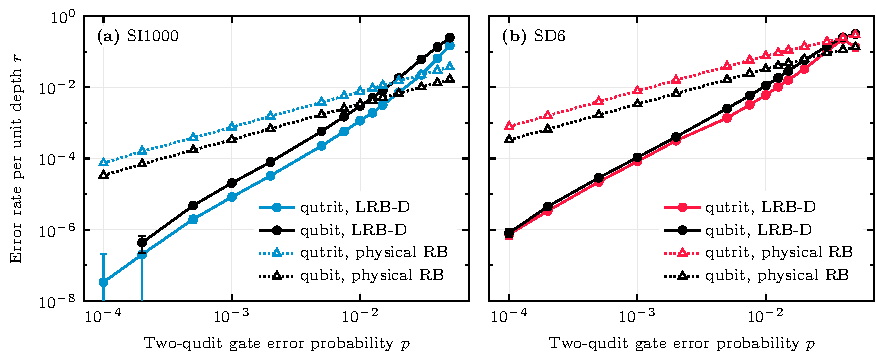
\includegraphics{figures/sdim140/lrb-vs-rb-k1-qubit-vs-qutrit.pdf}
  \caption{Fitted error rate per unit depth $r$ versus $p$ for the qutrit (colored) and qubit (black) $[[5,1,2]]$ codes in the one-ancilla layout under (a)~SI1000 and (b)~SD6: LRB-D with $k = 1$ (filled circles, solid lines) and physical RB of the same local dimension (white-filled triangles, dotted lines). The error rates are $r = 1 - \bar F = (q-1)(1-f)/q$ from Eq.~\eqref{eq:fbar} with local dimension $q$, so $r = 2(1-f)/3$ for the qutrit and $(1-f)/2$ for the qubit. The qutrit points are the one-ancilla points of \autoref{fig:four_configs}, and the qubit points come from the qubit production runs (\autoref{sub:qubit_code}). Error bars are central 68\% intervals of the parametric bootstrap (\autoref{sub:fit_model}); bars that are not visible are smaller than the markers, and the qutrit intervals that reach zero, under SI1000 at $p \le 2\times10^{-4}$, run to the bottom of the axis. The qubit SI1000 fit at $p = 10^{-4}$ returns zero error and is not drawn. From $p = 0.03$ on, the LRB-D fits rest on two or three depths. At every $p > 0$ the qubit RB error is $0.42$ to $0.48$ times the qutrit RB error. The qubit LRB-D error is $2.4$ to $2.7$ times the qutrit one under SI1000 for $5\times10^{-4} \le p \le 0.02$, and under SD6 it is $1.1$ to $1.3$ times the qutrit one for $p \le 2\times10^{-3}$ and $1.8$ to $1.9$ times for $5\times10^{-3} \le p \le 0.02$.}
  \label{fig:k1_qubit_qutrit}
\end{figure}

The encoded circuits behave the other way (\autoref{fig:k1_qubit_qutrit}). At every $p$ from $2\times10^{-4}$ to $0.015$, in both layouts and for $k = 1$ to $4$, the qubit LRB-D error per unit depth is the larger one. In the production runs from $p = 10^{-3}$ to $10^{-2}$ it is 2.4 to 3.0 times the qutrit error under SI1000 and 1.3 to 2.1 times under SD6. At larger $p$, where the fits rest on few depths, the ratio falls below one for some configurations with $k \ge 2$. With one ancilla and $k = 1$ at $p = 5\times10^{-3}$, for example, the LRB-D error under SI1000 is $5.8\times10^{-4}$ for the qubit and $2.3\times10^{-4}$ for the qutrit, while the RB errors are $1.7\times10^{-3}$ and $3.8\times10^{-3}$. Under SD6 the LRB-D errors are $2.6\times10^{-3}$ and $1.4\times10^{-3}$ and the RB errors $1.7\times10^{-2}$ and $3.9\times10^{-2}$. Both the RB and the LRB-D ratios compare average infidelities $r = (q-1)(1-f)/q$; in terms of $1 - f$ they would be $4/3$ larger, which changes neither the direction of either effect nor any $p^\star$, since a pseudo-threshold compares two error rates of the same local dimension. The acceptance is similar in the two codes: under SI1000 at $p = 5\times10^{-3}$ with one ancilla and $k = 1$, the qubit code rejects 60\% of the shots at $m = 2$ and 97\% at $m = 10$, against 63\% and 98\% for the qutrit code (\autoref{sub:postselection_cost}).

We have not identified the mechanism behind the larger encoded qubit error. The check rounds are the same circuits in both campaigns, with the same noise locations and the same total fault probability at each location, which the qubit channels spread over 3 and 15 non-identity Paulis instead of 8 and 80. The logical Cliffords are built from the same physical gates, and a qubit logical Clifford applies fewer of them, on average $8.2$ one-qubit and $1.5$ two-qubit gates against $16.8$ one-qutrit and $3.2$ two-qutrit gates. Why these circuits leave a larger postselected logical error for the qubit, and why the excess is larger under SI1000 than under SD6, remains open. The lower qubit pseudo-thresholds thus combine two measured effects: a physical baseline with fewer, slightly less noisy gates per Clifford and therefore a lower error, and a higher encoded error per unit depth.
